\documentclass[12pt]{report}
\newcommand\tab[1][.60cm]{\hspace*{#1}}
\usepackage{amsmath}
\usepackage{amsthm}
\usepackage[T1]{fontenc}
\usepackage{times}
\usepackage{pgfplots}
\pgfplotsset{compat = newest}
\usetikzlibrary{positioning, arrows.meta}
\usepgfplotslibrary{fillbetween}
\usepackage{lmodern}
\usepackage{ragged2e}
\usepackage{multicol, caption, booktabs}
\usepackage[flushleft]{threeparttable}
\usepackage[utf8]{inputenc}
\usepackage{siunitx}
\usepackage{setspace}
\usepackage[export]{adjustbox}
%\usepackage[usenames,dvipsnames]{xcolor}
\usepackage[affil-it]{authblk} 
\setlength{\columnsep}{1cm}
\newcommand{\dd}[1]{\mathrm{d}#1}
\usepackage[portrait, margin=1in]{geometry}
\graphicspath{ {C:/Users/Stu Lucko/Documents/GitHub/22SP_6103_11T_iDM/} }
\graphicspath{ {C:/Users/Stu Lucko/Documents/GitHub/Econometrics/} }
\graphicspath{ {C:/Users/Stu Lucko/Documents/GitHub/T4-Housing-Price-Index/} }
\newenvironment{Figure}
{\par\medskip\noindent\minipage{\linewidth}}
{\endminipage\par\medskip}
\usepackage{amssymb}
\usetikzlibrary{calc} 
%\onehalfspacing%
\usepackage{booktabs}
\usepackage{multirow}
\usepackage{siunitx}
\usepackage{fancyhdr}
\usepackage{lastpage}
\onehalfspacing


\pagestyle{fancy}
\fancyhf{}

\rfoot{Page \thepage \hspace{1pt} of \pageref{LastPage}}
\begin{document}


\title{%
Do Homes Located Near a Metro Station Incur a Price Premium? \thanks{{We would like to thank Professor Lo for his help in calculating the haversine distances.}} \\ 
\Large
Evidence from Washington, DC}
\author{Aru Gupta, Dylan Lucko, Yashwant Sai Devisetti \\ Professor Lo\\The George Washington University\\ \text{arugupta17@gwmail.gwu.edu} \\ \text{dylanlucko@gwu.edu} \\ \text{yaswanthsaidevisetti@gmail.com} \\ \text{https://github.com/Yaswanthd9/T4-Housing-Price-Index}}
\date{29 April 2022}
\maketitle
\begin{abstract}
\smallskip
This paper investigates how much more consumers are willing to pay for a home located within walking distance to a metro station in Washington, D.C. Goebel \emph{et al.} (2012), among other studies, find that consumers are willing to pay more for convenient goods and services. Living close to a metro simplifies employees' morning commutes and makes for a more convenient trip to and from the office. Based on theories of demand and scarcity, this paper hypothesizes that homes located within walking distance to a metro station will incur a price premium relative to homes farther away. Drawing from Freddie Mac (2019), we define "walking distance" as a half of a mile. Based on 2017 home sales in Washington, D.C., this paper utilizes a multiple linear regression with a distance dummy variable to estimate the price premium of homes within the half-mile radius. This paper predicts that homes located within walking distance of a metro station are 21\% more expensive than homes outside the radius.

\end{abstract}

\section*{Introduction}
Washington, DC boasts a wide range of employment opportunities in both the federal government and private sector. In 2017, about 530,000 individuals worked within DC's 43,000 firms, agencies, and establishments.\\
\tab With so many employees traveling to work each morning, individuals seek the best commuting method. Whereas commuting by car often leads to traffic delays, taking the DC metro offers a reprieve from the highway gridlock. Many workers take the metro nearest to their home to popular working destinations within the District, like Federal Triangle, Capitol Hill, and L'Enfant Plaza.\\
\tab This paper investigates how much $more$ home purchasers are willing to pay in order to live close to a metro station. If a metro station is within walking distance, e.g., a half mile, individuals can easily access the metro system. For employees living far away from a station, traveling to the station itself complicates their morning routine. 


\section*{Theory}
This paper utilizes two economic theories to analyze whether homes close to a metro station incur a price premium in Washington, DC: the law of demand and the theory of scarcity. The law of demand contends that as consumers demand more of a good, the price generally rises because supply curves are upward sloping\footnote{Please see Figures 11 and 12 in Appendix A}.\\ \tab In the case of buying a home in a convenient location, many buyers compete against each other in the marketplace. The individual who offers the most money for a home gets to buy it- so purchasers try to outbid one another- driving up the price.\\ \tab When demand rises for goods like phones, cars, or computers, firms generally increase the number of goods produced. In a city like Washington, however, home builders cannot simply build more houses to keep up with demand. The number of homes in convenient locations is scarce- there are only a finite number.\\
\tab There are a few elements to think about while evaluating a house. A house's allure is impacted by its area, trailed by its primary credits, including the number of rooms, bathrooms, land size, and proximity to amenities and schools in the area. To isolate the effect of living close to a metro station, this paper controls for many of the house's fixed effects.\\
\tab Drawing upon research from Freddie Mac- a federal mortgage lender- this paper contends that homes located within a half mile radius of a metro station are scarce. This paper also contends that individuals working within the District will demand homes closer to a metro than homes far away. Living within walking distance to a metro station simplifies the morning commute, and individuals often pay more for convenience. Since consumers demand a good (houses) that are scarce, we hypothesize that homes located within walking distance of a metro station will be more expensive than homes farther away. This paper defines walking distance as a half-mile.


\section*{Data}

To estimate the price premium incurred by consumers buying homes within a half mile radius of a metro station, data are obtained for Washington, DC home sales in 2017. Housing sale data are obtained for single family, multi family, and row- houses and synthesized via Kaggle. Metro location data are obtained from Open-Source DC. \\
\tab The dataset includes many home fixed effects, including the number of bathrooms, bedrooms, half bathrooms \& floors, the size of the home, the lot acreage, and the type of structure. The price of each home is demarcated in US dollars. Most importantly, each home pairs with a set of latitude and longitude coordinates. The dataset contains 12,399 homes sold in 2017. \\
\tab The dataset for Metro Locations contains variables indicating the lines running through the station and a pair of latitude and longitude coordinates for all 91 DC Metro stations.\\
\tab Based on the dataset, houses sold in 2017 for a median price of \$467,008 in the DC Metro Area. The mean distance to a metro station was a half mile, with the maximum distance falling around 2.5 miles. The average house had 6 rooms, 1.8 bathrooms, 1.23 kitchens, and 2 stories.\\
\tab In the modeling, the price of each home is the dependent variable. The parameter of interest is the coefficient on Metro.5, which is a dummy variable indicating whether a house falls within a half mile radius of one of the metro stations. The coefficient on Metro.5 indicates the price differential for a house loathed near a metro station. The other independent variables include the home fixed effects mentioned above. We control for home fixed effects to isolate the effect of living within a half mile radius of the metro station to ensure the independent variables are uncorrelated with the error term in the econometric models.\\
\tab The original dataset contained every home sale in Washington, DC for the years 1980-2019. We first separated the date column (dd-mm-yyyy) into three columns for day, month, and year of the sale. We then used Boolean operators to filter out all the homes sold in 2017.\\
\tab Performing exploratory data analysis indicated three outliers in the price variable, and those were removed. In fourth econometric model, this paper uses the natural logarithm of home price as the dependent variable. \\
\tab The variable for home structure originally used strings to demarcate the style of home, e.g., single. This paper converts the string names to integer values.\\
\tab To determine if a given house falls within a half mile radius to a metro station, the distance from each house to the nearest metro station must be calculated. To do so, this paper utilizes the haversine formula and the two pairs of latitude and longitude coordinates for each house and each metro station. Equation~\ref{eqn:1} illustrates how this paper calculates the distances.
\begin{gather}
\ d=2r\ arcsin \left(\sqrt{sin^{2} \left( \frac{\phi_{2}-\phi_{1}} {2} \right) +cos(\phi_1)cos(\phi_2)sin^2 \left( \frac{\lambda_{2}-\lambda_{1}} {2} \right) } \right) \
\label{eqn:1}
\end{gather}
where $\phi_1$ and $\phi_2$ correspond to latitude 1 and latitude 2, $\lambda_1$ and $\lambda_2$ correspond to longitude 1 and longitude 2, and $r$ is the radius of the Earth.\\
\tab Equation~\ref{eqn:15} indicates the process repeated for all 12,399 homes and 91 metro stations:
\begin{gather}
\ \phi_1 = \text{House\ 1\ Latitude} \nonumber\\
\phi_2 = \text{Metro\ 1\ Latitude} \nonumber\\
\lambda_1 = \text{House\ 1\ Longitude} \nonumber\\
\lambda_2 = \text{Metro\ 1\ Longitude}\ 
\label{eqn:15}
\end{gather}
\tab The latitude and longitude coordinates for each house and each metro station are substituted into the haversine function for $(\phi_1,\ \lambda_1) \ \& \ (\phi_2,\ \lambda_2)$ respectively. The distance from a single house to all 91 metro stations are
calculated, then the minimum distance is selected and added to the data frame. \\
\tab The haversine formula produces 91 distances for each house. Equation~\ref{eqn:2} finds the minimum distance for each house given the list of 91 distances.
\begin{gather}
\ \min{(distances\ _{1}^{91})} = Distance \ 
\label{eqn:2}
\end{gather}
\clearpage
Based on the minimum distance found using Equation~\ref{eqn:2}, dummy variables are found using Equation~\ref{eqn:3}.
\begin{gather}
\ 
Metro.5=
\begin{cases}
1 & \text{if } Distance \leq 0.50\\
0 & \text{if } Distance > 0.50
\end{cases}
\ 
\label{eqn:3}
\end{gather}

Now that each house has a dummy variable indicating whether it lies within a half mile radius of a metro station, this paper proceeds with Exploratory Data Analysis. 
\clearpage

\section*{Exploratory Data Analysis}
To demonstrate the usefulness of each variable in the model, an exploratory data analysis of the variable was conducted. 
\begin{figure}[h]
\begin{center}
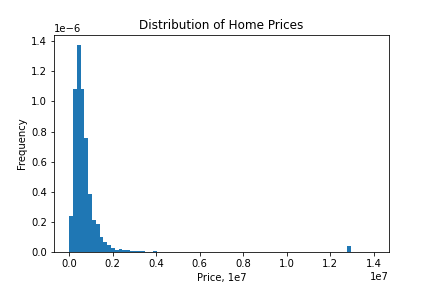
\includegraphics[width=130mm]{priceHist.png}
\end{center}
\caption{\textbf{The distribution of home prices in Washington, DC.}}
\label{fig:priceHist}
\end{figure}
\\
First, we examined the dependent variable, $Price$, to learn more about its distribution. The histogram for $Price$ that the price of homes in Washington, DC skews to the right. The histogram also showed a few outliers in the data that should be removed before conducting further analysis. 

\clearpage
\begin{figure}[h]
\begin{center}
\caption{\textbf{The distribution of home prices in Washington, DC, sans outliers.}}
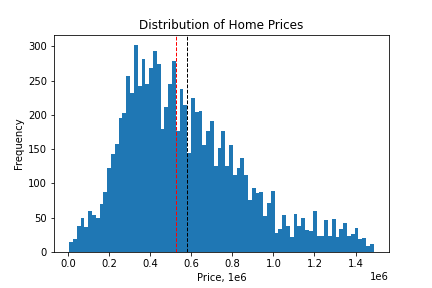
\includegraphics[width=130mm]{newPriceHist.png}
\end{center}
\label{fig:NewpriceHist}
\end{figure}
After removing the observations above $Q_3+(1.5*IQR)$, we create a new variable for price, newPrice. Even though the histogram for newPrice shows that the average price for homes in the DC area is higher than the median price, the new price data is now more normally distributed than before. This is key for meeting the multiple linear regression assumptions. The peaks in the newPrice histogram show that most homes range between two-hundred and eight-hundred thousand dollars. \\
\clearpage

\tab This paper theorizes that the price premium decreases as the distance between a home in Washington D.C. and the nearest metro station increases. The histogram below shows the distribution of the homes by their proximity to the nearest metro station.

\begin{figure}[h]
\begin{center}
\caption{\textbf{The distribution of homes based on their proximity to the nearest metro station}}
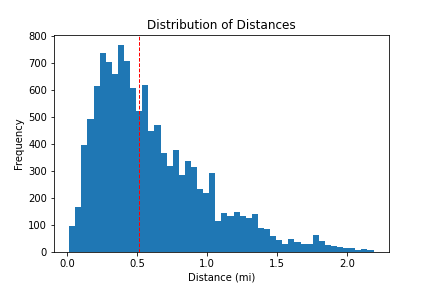
\includegraphics[width=130mm]{distanceHist.png}
\end{center}
\label{fig:distanceHist}
\end{figure}
As observed in the Distance histogram above, median homes are located within an $\approx$ 0.5-mile radius of the nearest metro station. The distribution is skewed to the right, with the distance ranging from zero to over two miles. Given that most homes are located within a one-mile radius, a dummy variable is created to see the difference in the price premium for homes within and outside the 0.5-mile radius to conduct further analysis.
\clearpage

\begin{figure}[h]
\begin{center}
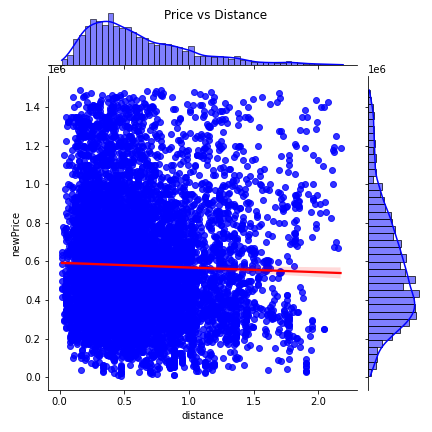
\includegraphics[width=110mm]{DistanceJoint.png}
\end{center}
\caption{\textbf{.}}
\label{fig:distanceJoint}
\end{figure}

The joint plot above shows the scatter plot of price vs distance and the associated distributions of distance on the top and price on the right. The linear model line of best fit in the scatterplot shows a clear downward sloping negative relationship between the two variables. The downward sloping trend line shows that as the distance increases, the price of the homes decreases. 
\clearpage

To take a deeper look into the factors that affect home prices, it is important to take fixed effects and features of the homes into account.
\begin{figure}[h]
\begin{center}
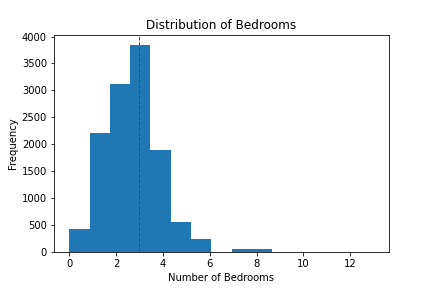
\includegraphics[width=130mm]{bedroomHist.png}
\end{center}
\caption{\textbf{Distribution of Bedrooms}}
\label{fig:bedHist}
\end{figure}
\\
\tab First, we looked at the number of bedrooms in the homes and their impact on price.
The histogram shows the median number of bedrooms for homes sold in 2017 to be 3. The number of bedrooms ranges from one to six, with eight bedrooms being an outlier.
\clearpage

\begin{figure}[h]
\begin{center}
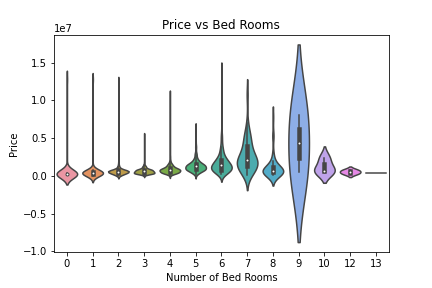
\includegraphics[width=130mm]{BedViolin.png}
\end{center}
\caption{\textbf{Distribution of price vs bedrooms}}
\label{fig:bedVio}
\end{figure}
When analyzing the variable bedrooms, it was expected that the price of the homes in D.C. would increase as the number of bedrooms increased. On the contrary, the white points in the violin plot show a steady increase in the median price as the number of bedrooms increases to five. At six bedrooms, the median price of homes begins to decline, and the price becomes constant at eight bedrooms. The distribution of bedrooms seen in Figure~\ref{fig:bedVio} helps this paper decide when to add quadratic terms to encapsulate marginal diminishing returns of adding additional bedrooms.
\clearpage


\begin{figure}[h]
\begin{center}
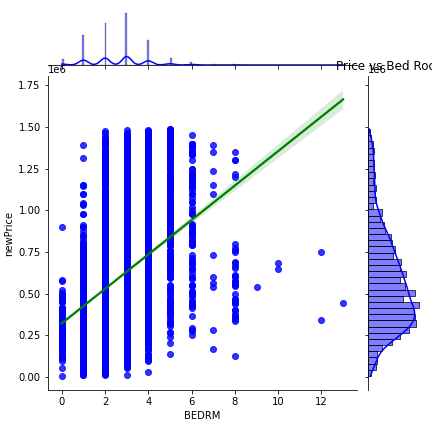
\includegraphics[width=130mm]{BedJoint.png}
\end{center}
\caption{\textbf{.}}
\label{fig:bedJoint}
\end{figure}
The joint plot for bedrooms and price shows the overall upward sloping linear model line of best fit, which indicates a positive relationship between price and the number of bedrooms. It is also observed that the price peaks at around four-hundred thousand dollars in relation to the number of bedrooms. 
\clearpage

\begin{figure}[h]
\begin{center}
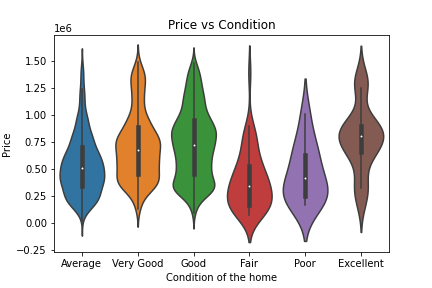
\includegraphics[width=130mm]{ConditionViolin.png}
\end{center}
\caption{\textbf{.}}
\label{fig:cndVio}
\end{figure}
The violin plot shows the home prices by condition for houses within the half-mile radius of the nearest metro station in orange and outside the radius in blue. Overall, the violin plot shows that homes within a half-mile radius are typically priced higher regardless of the listed condition. Contrary to expectations, the violin plot shows that the median home prices for homes listed as “Fair” are priced the lowest, and those listed as “Good” have a higher price than those listed as “Very Good.” 

The width of the violin plots also indicates that more “Excellent” homes were sold at a high price. The violin plot ultimately shows that individuals pay higher for a lower condition home if living close to the metro station. 
\clearpage


\begin{figure}[h]
\begin{center}
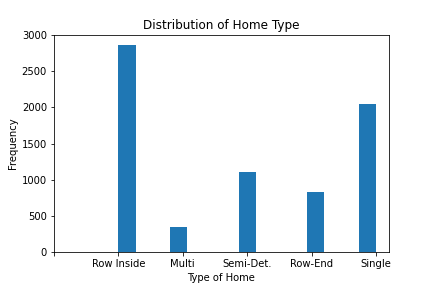
\includegraphics[width=130mm]{structureHist.png}
\end{center}
\caption{\textbf{.}}
\label{fig:strHist}
\end{figure}
This research takes into account the price difference between different styles and structures of homes. The histogram shows that most homes in the dataset are categorized as "Row Inside", followed by “Single” and “Multi” being the least frequent. 
\clearpage
\begin{figure}[h]
\begin{center}
\caption{\textbf{Price vs structure, split for distance to metro. Recall 1 means living within a half-mile radius and 0 means living outside a half-mile radius. }}
\includegraphics[width=130mm]{structureViolin.png}
\end{center}
\label{fig:strHist}
\end{figure}
The violin chart shows that the median price for “Row Inside” homes is the highest. The violin for this structure is wider for homes within a half-mile radius. The width of the “Row End” violin shows that it is the most popular structure among the houses in a half-mile radius.\\
\tab Figure~\ref{fig:strHist} illustrates that the individuals living in different styled houses demand metro access differently. As seen above, individuals living within Row Inside, Multi Family, and Row End incur a higher price for living within a half-mile to a metro station, while those living in a Single or Semi Detached pay less.

\clearpage

\section*{Econometric Specification}
This paper utilizes a multiple linear regression approach using ordinary least squares estimators to predict if homes located within a half mile radius of a metro station incur a price premium. It is natural for homes to differ in price for several reasons, including size, year built, geographical location, or number of bedrooms. To determine if the metro station proximity is responsible for the differences in price, this paper controls for many home fixed effects mentioned above and in the data section.\\ \\
\tab This paper estimates four models, the first three utilize the price of a home as the dependent variable, denoted in dollars. The fourth equation estimates the price premium using the log of the home price to account for skew in the home price data. The general specification of the four models take on the functional form of Equation~\ref{eqn:1}.
\begin{align}
\ price = \beta_0 +\delta_1\ metro.5 + \beta_k\ (house\ fixed\ effects )+ u \ 
\label{eqn:1}
\end{align}
where $\delta_1$ is the parameter of interest and denotes the price differential for a house located within a half mile radius and a house located outside the radius. $metro.5$ is a dummy variable denoting whether a house falls within the radius: $metro.5$=1 if the house lies within the half mile radius and $metro.5$=0 if else.\\ \\
\tab The term house fixed effects encompass the home attributes that do not change on average, including the number of bathrooms \& half-bathrooms, the lot size, the number rooms, the number of kitchens, and the type of structure.\\ \\
\tab In Model 4, this paper performs a stepwise selection process to determine which of the nine home fixed effects should be included in the final model. The stepwise selection independently estimates $price$ as a function of the nine home fixed effects and the $metro.5$ variable for a total of ten regressions. The term with the highest $R^2$ is added to the model, we call this $variable1$. Next, nine regressions are run, each with $variable1$ and the other eight variables; the term with the highest $R^2$ is added, we call this $variable2$. This process is repeated, adding the variable that results in the highest $R^2$ and removing variables that are not statistically significant. Model 4, estimates $\text{(log)}price$ as a function of the variables chosen by this method. \\ \\
\tab We expect the sign on $metro.5$ to be positive and moderately large as this paper hypothesizes that homes located within the half mile radius will be more expensive. We also expect the signs on $bedrooms$, $bathrooms$, $size$, $landarea$ to all be positive, indicating a higher price given more of these home attributes. We expect some of the structures to have a positive sign and others to have a negative sign, based on the style and quality of the structure. The results of the four regression models can be found in the next section.\\ \\
\tab To eliminate any multicollinearity issues, this paper examines a correlation matrix to identify independent variables that correlate with one another. Table~\ref{} illustrates the correlation matrix, with high values denoted in red.
\begin{table}[h!]
\centering
\begin{tabular}{|c| c | c |c |c |c |c |c | c | c|} 
\hline
\multicolumn{10}{|c|}{ \textbf{Correlation Matrix}} \\
\hline\hline
&$\text{(log)}price$& Price& struc. & metro50& Stories& Land& Bath& Rooms& Half\\[0.5ex] \hline \ 
$\text{(log)}price$& 1& 0.917& -0.074& 0.048& 0.170& 0.158& 0.480 & 0.357& 0.321\\ [0.5ex]\hline \ 
Price& 0.917& 1&-0.040& 0.031& 0.199& 0.205& \textbf{\color{red}{0.524}}& 0.389& 0.348\\ [0.5ex]\hline\ 
sruc.& -0.074& -0.040 & 1& -0.146& -0.042 & \textbf{\color{red}{0.505}}& 0.136& 0.095& 0.099 \\ [0.5ex]\hline \ 
metro50& 0.048 & 0.031&-0.146& 1& 0.014& -0.177& -0.099& -0.170& -0.1050\\ [0.5ex] \hline \ 
Stories& 0.170 & 0.199&-0.042& 0.014& 1& -0.025& 0.033& 0.030& 0.031\\ [0.5ex]\hline \ 
Land& 0.158& 0.205&\textbf{\color{red}{0.505}}& -0.177& -0.025& 1& 0.420 & \textbf{\color{red}{0.505}}& 0.306\\ [0.5ex] \hline \ 
Bath& 0.480& \textbf{\color{red}{0.524}}&0.136& -0.099& 0.033& 0.420&1& \textbf{\color{red}{0.694}}& 0.290\\ [0.5ex]\hline \ 
Rooms& 0.357& 0.389&0.095 & -0.170& 0.030& \textbf{\color{red}{0.506}}& \textbf{\color{red}{0.694}}& 1& 0.396 \\ [0.5ex]\hline \ 
Half& 0.321& 0.348&0.099& -0.105& 0.031& 0.306& 0.290& 0.3963& 1 \\ [0.5ex]\hline
\hline
\end{tabular}
\caption{\footnotesize Values above 0.50 are highlighted in red. Note that the correlation between log(price) and Price are not considered as they do not appear in the same model.}
\label{table:1}
\end{table}

\section*{Results}
This paper utilizes a multiple linear regression approach using ordinary least squares estimators to predict if homes located within a half- mile radius incur a price premium relative to homes outside of the half- mile radius.\\
\tab This paper estimates four different econometric models but will only discuss the results of the two consequential models, Model 1 and Model 4. Details about all four models are found in the Econometric Specification Section.\\
\tab The first prediction framework estimates the price differential for houses inside and outside of the half-mile radius without controlling for the home's fixed effects, denoted by Equation~\ref{eqn:4}.
\begin{align}
\ price = \beta_0 +\delta_1\ metro.5 + u \ 
\label{eqn:4}
\end{align}
The reported coefficients on $\hat{\delta_1}$ in Column (1) of Table~\ref{table:2} is 24,776.83 and it is statistically significant. This means that a house falling within a half mile radius of a metro station is associated with a \$24,778 price premium, all else equal.\\
\tab Notice, however, that the $R^2$ reported at the bottom of Column (1) is 0.001. This means that about 1\% of the sample variation in price can be explained by the distance dummy variable. Therefore, a more sophisticated model must include home fixed effects.\\
\tab The second and third prediction models are included to demonstrate the thought process followed by this paper. We estimate a general linear model first (Model 2) to relax the econometric assumptions in attempt to solve multicollinearity issues. Model 3 uses ordinary least squares and robust standard errors to solve heteroskedasticity issues. The variables included in Model 2 and Model 3 can be found in Column (2) and Column (3) of Table~\ref{table:2}. These home fixed effects are chosen rather arbitrarily, and subsequently, result in very strong multicollinearity issues. As a result, Model 4 employs a stepwise selection process to better choose the home fixed effects and therefore reduces multicollinearity issues. \\
\tab The fourth prediction framework estimates the price differential for houses inside and outside of the half-mile radius, controlling for the home's fixed effects, denoted by Equation~\ref{eqn:5}.
\begin{align}
\ \text{log}(price) = \beta_0 +\delta_1\ metro.5 + \beta_1 \ rooms + \beta_2\ rooms^2 + \beta_3\ bathrooms \nonumber \\ + \beta_4\ HalfBath + \beta_5\ bedrooms + \beta_6\ bed^2 + \beta_6\ structure + u \ 
\label{eqn:5}
\end{align}
The quadratic terms on $rooms$ and $bedrooms$ allows for diminishing marginal returns to each of these home attributes. The stepwise selection process and joint F tests for inclusion indicate a stronger $R^2$ when including the quadratic terms as it corrects the model for better functional form. \\
\tab The reported coefficient, $\hat{\delta_1}$ in Column (4) of Table~\ref{table:2}, is 0.21 and it is statistically significant. This means that a home located within a half-mile of a metro station is associated with a 21\% higher price than homes located outside of the radius. \\
\tab Furthermore, the coefficients on bedrooms and bathrooms are positive while their corresponding quadratic terms are negative. All four terms are statistically significant. This means that adding a bedroom or bathroom to a house increases its price but only up to a point. If too many bedrooms or bathrooms are added, the price begins to fall. This is confirmed graphically in Figure~\ref{fig:bedVio}.\\ \tab For all of the regression models above, the t-statistics use robust standard errors. Based on the residual analysis in Figures 13 and 14, there is evidence for heteroskedasticity. Therefore, robust standard errors mitigate this issue and allow t-statistics to be used in determining if coefficients are significant. 












\begin{table}[h!]
\centering
\begin{threeparttable}

\caption{Effects of Metro Proximity on Home Prices}
\begin{tabular}{lccccc} 
%\multicolumn{6}{c}{ \textbf{DinD Treatment Effects on NOx}} \\
\hline\hline\\[0.001ex]
& \multicolumn{4}{c}{$Price$} & \multicolumn{1}{c}{Log($Price$)} \\ [0.1ex] \cline{2-4} \cline{6-6} 
\\[0.001ex]
& (1) & (2) & (3) && (4) \\ [0.5ex] 
\hline \\[0.1ex]
Intercept& 574364.70\footnotesize***& 189648.32\footnotesize***& 248707.05&& 17.70\footnotesize*** \\
& \footnotesize[-3424.27]& \footnotesize(19850.63)& \footnotesize(263607.00)&& \footnotesize[0.10] \\
metro50& 24776.83\footnotesize***& 97631.25\footnotesize***& 96892.24\footnotesize***&& 0.21\footnotesize*** \\
& \footnotesize[8176.48]& \footnotesize(12838.28)& \footnotesize(12821.84)&& \footnotesize[0.03] \\
Stories& & 63388.06\footnotesize***& 64507.54\footnotesize***&& \textemdash \\
& & \footnotesize(8460.41)& \footnotesize(8447.44) && \\
Land& & 7.84\footnotesize***& 9.04&& \textemdash \\
& & \footnotesize(2.52)& \footnotesize(2.53)& & \\
Bedroom& & 150960.90\footnotesize***& 143963.93\footnotesize***&& 0.32\footnotesize*** \\
& & \footnotesize(4490.45)& \footnotesize(4717.21)&& \footnotesize[0.01]\\
Half& & 94667.83\footnotesize***& 87127.34\footnotesize***&& 0.24\footnotesize*** \\
& & \footnotesize(6886.83)& \footnotesize(7053.45)&& \footnotesize([0.02]\\
Multi& & -331169.10\footnotesize***& -309597.28\footnotesize***&& -0.78\footnotesize*** \\
& & \footnotesize(18996.8)2& \footnotesize(19493.71)&& \footnotesize[0.06] \\
Detached& & -190811.19\footnotesize***& -197509.55\footnotesize***&& -0.54\footnotesize*** \\
& & \footnotesize(11459.7)8& \footnotesize(11522.49)&& \footnotesize[0.03] \\
Row& & -52120.28\footnotesize***& -57029.36\footnotesize***&& -0.17\footnotesize*** \\
& & \footnotesize(12490.2)4& \footnotesize(12507.49)&& \footnotesize[0.03] \\
Single& & -77761.28\footnotesize***& -83945.82\footnotesize***&& -0.25\footnotesize*** \\
& & \footnotesize(13528.3)0& \footnotesize(13562.47)&& \footnotesize[0.03]\\
Rooms& & & && 0.16\footnotesize***\\
& & & && \footnotesize[0.02] \\
$Rooms^2$& & & && -0.011\footnotesize*** \\
& & & && \footnotesize[0.00] \\
$Bed^2$& & & && -0.005\footnotesize*** \\
& & && & \footnotesize[0.00] \\
Fixed Effects & Yes& Yes & Yes & & Yes \\ [0.5ex]
Stepwise & No& No & No & & Yes \\ [0.5ex]
Observations& 9176 & 4825& 4825 && 4834 \\ [0.5ex]
$R^2$ & 0.001 & 0.381& 0.327 && 0.321 \\ [0.5ex]
Adj-$R^2$& 0.001& & 0.326 & & 0.320 \\ [0.5ex]
\hline
\bottomrule
\end{tabular}
\begin{tablenotes}
\item \footnotesize{Notes. Each column reports results from a regression of dummy variables and other indicators for $Price$. Column (1), Column (2), and Column (3) use the price of homes denoted in US dollars while Column (4) uses the log($Price$) as the dependent variable. Fixed effects include attributes to the homes that do not vary with time. Model 2 uses a general linear model while Model 1, 3, and 4 use ordinary least squares. The standard errors reported in square brackets are robust standard errors. HC3 covariance methods are used in the ols model in python ($cov_type='HC3'$). Stepwise indicates if stepwise selection was performed. $***p<.01. **<.05. *p<.10.$}

\end{tablenotes}
\label{table:2}
\end{threeparttable}
\end{table}
\clearpage


\section*{Further Research}

Based on the fact that the $R^2$ of Model 4- which includes the home's fixed effects, quadratic and logarithmic terms to fix functional form misspecification, and stepwise selection- only captures 32\% of the sample variation in price, it is clear that additional independent variables ought to be added to the model. Since this research strictly focuses on the fixed effects of the homes sold in Washington, D.C., in 2017, we contend that factors such as crime rate, median household income, and other economic considerations could strengthen the analysis. \\
\tab To further this research, it would be beneficial to incorporate the difference in the price premium in different wards of the district. This will help gain a deeper understanding of the different neighborhoods in D.C. Studying the proximity to different metro lines will also provide a greater understanding of the house price premium in different neighborhoods. 

\section*{Concluding Remarks}
Through our analysis, we can conclude that homebuyers within the half-mile radius of the nearest metro station pay a price premium of 21\% which is greater than for homes beyond the half-mile radius by 21\%. The exploratory data analysis of the fixed effects and the data model including the variables for fixed effects and their quadratic forms show that homebuyers paid a higher price when living within a half-mile radius regardless of the number of bathrooms and bedrooms. We also found that homebuyers paid a higher premium for a lower condition home if the home was in close proximity to a metro station. 
\clearpage

\section*{Appendix A}
\begin{multicols}{2}

\begin{center}
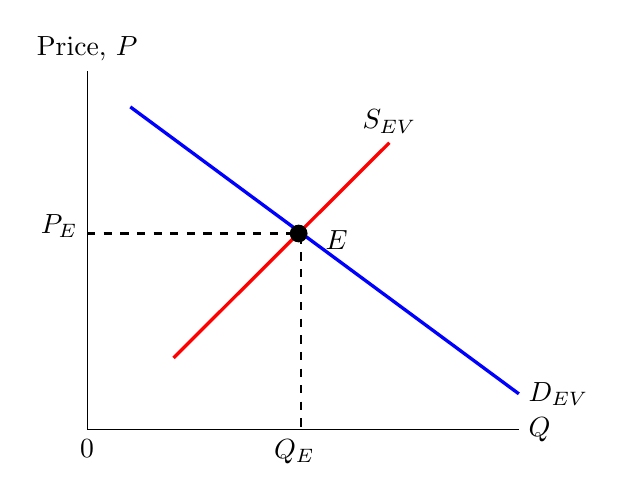
\begin{tikzpicture}
\begin{axis}[
scale = .8,
xmin = 0, xmax = 10,
ymin = 0, ymax = 10,
axis lines* = left,
xtick = {0}, ytick = \empty,
axis on top,
clip = false,
]
% Colouring areas
%\fill[orange, opacity = 0.1] (0, 7.67) -- (0, 3.67) -- (5.5, 3.67) -- (5.5, 7.67);
%\fill[green, opacity = 0.1] (5.5, 0) -- (5.5, 3.67) -- (7, 3.67) -- (7, 0);

% Supply and demand curves
\addplot[color = blue, very thick] coordinates {(1,9) (10,1)};
\addplot[color = red, very thick] coordinates {(2,2) (7,8)};
%\addplot[color = red, opacity = 0.5, very thick] coordinates {(6,1) (9,9)};

% Dashed lines
\addplot[color = black, dashed, thick] coordinates {(0, 5.47) (4.95, 5.47) (4.95, 0)};
%\addplot[color = black, dashed, thick] coordinates {(0, 3.67) (7, 3.67) (7, 0)};

% Coordinate points
\addplot[color = black, mark = *, only marks, mark size = 3pt] coordinates {(4.9, 5.47)};

% Labels
\node [right] at (current axis.right of origin){$Q$};
\node [above] at (current axis.above origin) {Price, $P$};
\node [right] at (5.3, 5.3) {$E$};
%\node [right] at (7, 3.67) {$E^\prime$};
\node [right] at (10, 1) {$D_{EV}$};
\node [above] at (7, 8) {$S_{EV}$};
%\node [right] at (9, 9) {$S^\prime$};
\node [left] at (0, 5.67) {$P_E$};
%\node [left] at (0, 3.67) {$P^\prime$};
\node [below] at (4.8, 0) {$Q_E$};
%\node [below] at (7, 0) {$Q^\prime$};


% Arrows
%\draw[-{Triangle[length = 4mm, width = 2mm]}, red, opacity = 0.3] (6.3, 8.5) to (8.3, 8.5);
%\draw[-Triangle] (5, 11) to [out = 180, in = 90] (2, 6);
%\draw[-Triangle] (10, -1.5) to [out = 90, in = 0] (6.5, 0.7);

\end{axis}
\end{tikzpicture}
\end{center}

\begin{center}
\emph{Figure 11}\\
\end{center}
%%%%%

\begin{center}
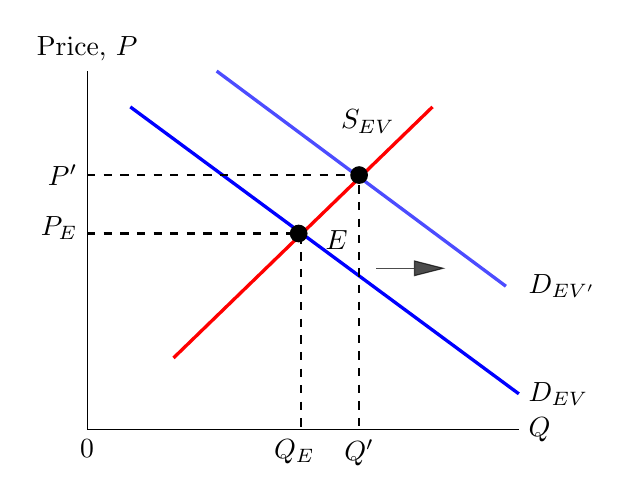
\begin{tikzpicture}
\begin{axis}[
scale = .8,
xmin = 0, xmax = 10,
ymin = 0, ymax = 10,
axis lines* = left,
xtick = {0}, ytick = \empty,
axis on top,
clip = false,
]
% Colouring areas
%\fill[orange, opacity = 0.1] (0, 7.67) -- (0, 3.67) -- (5.5, 3.67) -- (5.5, 7.67);
%\fill[green, opacity = 0.1] (5.5, 0) -- (5.5, 3.67) -- (7, 3.67) -- (7, 0);

% Supply and demand curves
\addplot[color = blue, very thick] coordinates {(1,9) (10,1)};
\addplot[color = blue, very thick, opacity = 0.7] coordinates {(3,10) (9.7,4)};
\addplot[color = red, very thick] coordinates {(2,2) (8,9)};
%\addplot[color = red, opacity = 0.5, very thick] coordinates {(6,1) (9,9)};

% Dashed lines
\addplot[color = black, dashed, thick] coordinates {(0, 5.47) (4.95, 5.47) (4.95, 0)};
\addplot[color = black, dashed, thick] coordinates {(0, 7.1) (6.3, 7.1) (6.3, 0)};

% Coordinate points
\addplot[color = black, mark = *, only marks, mark size = 3pt] coordinates {(4.9, 5.47)};
\addplot[color = black, mark = *, only marks, mark size = 3pt] coordinates {(6.3, 7.1)};

% Labels
\node [right] at (current axis.right of origin){$Q$};
\node [above] at (current axis.above origin) {Price, $P$};
\node [right] at (5.3, 5.3) {$E$};
%\node [right] at (7, 3.67) {$E^\prime$};
\node [right] at (10, 1) {$D_{EV}$};
\node [right] at (10, 4) {$D_{EV^\prime}$};
\node [above] at (6.5, 8) {$S_{EV}$};
%\node [right] at (9, 9) {$S^\prime$};
\node [left] at (0, 5.62) {$P_E$};
\node [left] at (0, 7.1) {$P^\prime$};
\node [below] at (4.8, 0) {$Q_E$};
\node [below] at (6.3, 0) {$Q^\prime$};


% Arrows
\draw[-{Triangle[length = 4mm, width = 2mm]}, black, opacity = 0.7] (6.7, 4.5) to (8.3, 4.5);
%\draw[-Triangle] (5, 11) to [out = 180, in = 90] (2, 6);
%\draw[-Triangle] (10, -1.5) to [out = 90, in = 0] (6.5, 0.7);

\end{axis}
\end{tikzpicture}
\end{center}

\begin{center}
\emph{Figure 12}\\
\end{center}
\end{multicols}
Increased demand for housing shifts the demand curve to the right, increasing the price.

\section*{Appendix B}
\begin{multicols}{2}
\begin{Figure}
\centering
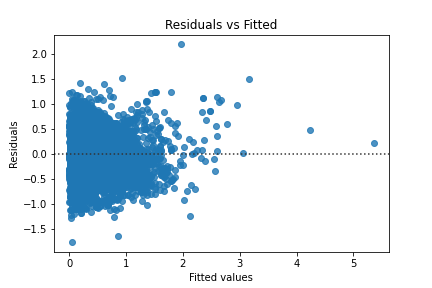
\includegraphics[width=\linewidth]{resid.png}
%\captionof{figure}{my caption of the figure}
\end{Figure}
\begin{center}
\emph{Figure 13}\\
\end{center}

\begin{Figure}
\centering
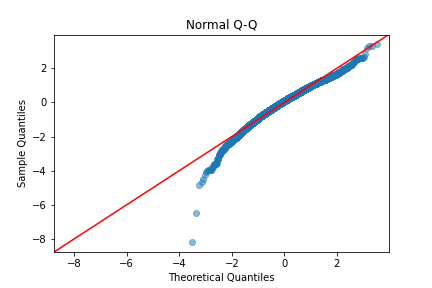
\includegraphics[width=\linewidth]{normalqq.png}
%\captionof{figure}{my caption of the figure}
\end{Figure}
\begin{center}
\emph{Figure 14}\\
\end{center}
\end{multicols}
\clearpage


\section*{References}

\tab Christopher Correa. (2018, July 30). Preparing the D.C. Real Property Dataset. Kaggle. Retrieved April 28, 2022, from https://www.kaggle.com/code/christophercorrea/preparing-the-d-c-real-property-dataset/dataOpen source DC\\

Lerner, M. (2019, October 2). Want to buy a home near a metro station? here's how much it will cost you. The Washington Post. Retrieved April 28, 2022, from https://www.washingtonpost.com/business/2019/10/03/want-buy-home-near-metro-station-heres-how-much-it-will-cost-you/\\

Proximity to a Metro Rail station and its impact on Washington, DC metropolitan house prices: Amenity or not? Freddie Mac. (n.d.). Retrieved April 28, 2022, from https://www.freddiemac.com/research/insight/20191002-metro-station-impact\\





\end{document}
